\section{Introducción}

En esta práctica se aborda el diseño de controladores mediante la técnica de \textbf{ubicación arbitraria de polos}, un método fundamental en el análisis y síntesis de sistemas de control en el espacio de estados. El propósito principal es modificar la dinámica de una planta determinada para que el sistema en lazo cerrado cumpla con \textit{especificaciones deseadas de respuesta transitoria}, tales como el tiempo de establecimiento y el coeficiente de amortiguamiento.

A través del cálculo de las matrices del sistema, su discretización e implementación en un \textbf{controlador digital basado en el PSoC}, se busca comprender cómo la realimentación de estados permite alterar el comportamiento dinámico y mejorar el desempeño del sistema. 

Finalmente, se comparan los resultados obtenidos mediante simulación en \texttt{MATLAB} con los resultados experimentales, analizando la efectividad del diseño y las posibles diferencias entre el modelo teórico y la práctica.

\section*{Objetivos}

\begin{itemize}
	\item Diseñar un controlador que modifique la dinámica de la planta para satisfacer condiciones específicas de la respuesta transitoria del sistema de control en lazo cerrado.
	\item Asegurar que el sistema regulado sea estable.
	\item Observar y analizar los efectos del controlador en el comportamiento dinámico del sistema.
	\item Considerar distintos métodos para el ajuste de los parámetros del controlador y analizar los resultados obtenidos.
	\item Diseñar el sistema de control en \texttt{MATLAB} e implementar la ecuación en diferencia correspondiente en el \texttt{PSoC}.
\end{itemize}



\documentclass{standalone}
\usepackage{tikz}
\usetikzlibrary{arrows.meta, positioning}

\begin{document}
	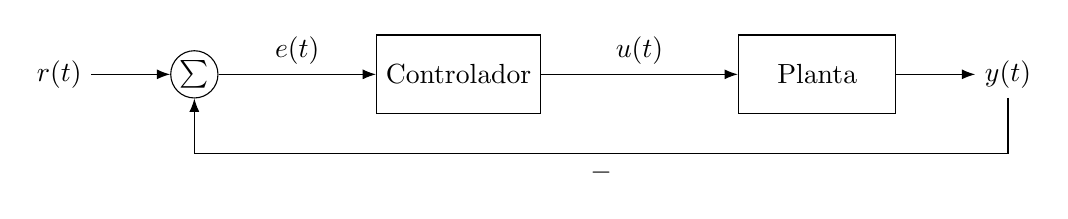
\begin{tikzpicture}[
		block/.style = {draw, rectangle, minimum height=1cm, minimum width=2cm, align=center},
		sum/.style = {draw, circle, inner sep=0pt, minimum size=6mm},
		>={Latex}
		]
		% Bloques
		\node[block] (plant) {Planta};
		\node[block, left=of plant, xshift=-1.5cm] (controller) {Controlador};
		\node[sum, left=of controller, xshift=-1cm] (sum) {$\sum$};
		\node[left=of sum] (ref) {$r(t)$};
		\node[right=of plant] (output) {$y(t)$};
		
		% Conexiones
		\draw[->] (ref) -- (sum);
		\draw[->] (sum) -- node[above] {$e(t)$} (controller);
		\draw[->] (controller) -- node[above] {$u(t)$} (plant);
		\draw[->] (plant) -- (output);
		\draw[->] (output) |- ++(0,-1) -| node[pos=0.25, below] {$-$} (sum.south);
	\end{tikzpicture}
\end{document}
